\documentclass[c]{beamer}

\usepackage{graphicx}
\usepackage{epsfig}
\usepackage{hyperref}
\usepackage{booktabs, caption}
\usepackage{anyfontsize}
\usepackage{ucs}
\usepackage[ngerman]{babel}

% suppress navigation bar
\beamertemplatenavigationsymbolsempty

\mode<presentation>
{
  \usetheme{jd}
  \setbeamercovered{transparent}
  \setbeamertemplate{items}[circle]
}

% set fonts
\usepackage{fontspec}
\setsansfont{Changa One}
\setbeamerfont{frametitle}{size=\LARGE,series=\bfseries}

\usepackage{setspace}
\setstretch{3}
\parindent 0pt

% color definitions
\usepackage{color}
\definecolor{uipoppy}{RGB}{225, 64, 5}
\definecolor{uipaleblue}{RGB}{96,123,139}
\definecolor{uiblack}{RGB}{0, 0, 0}
\definecolor{uigreen}{RGB}{96, 147, 115}%{0,125, 113} 
\definecolor{uigreen_dark}{RGB}{31, 39, 42}
\definecolor{uigray}{RGB}{217, 217, 217}
\definecolor{uigray2}{RGB}{117, 117, 117}
\definecolor{uired}{RGB}{187, 114, 101}

%\definecolor{blue1}{RGB}{41, 128, 185}
%\definecolor{blue2}{RGB}{52, 152, 219}
%\definecolor{blue2}{RGB}{174, 198, 207}
\definecolor{blue2}{RGB}{119, 158, 203}

\definecolor{blue1}{RGB}{83, 104, 114}

\definecolor{blue3}{RGB}{44, 62, 80}
\definecolor{turquoise}{RGB}{22, 160, 133}
\definecolor{green1}{RGB}{0,125, 113}

%\definecolor{yellow1}{RGB}{241, 196, 15}
\definecolor{yellow1}{RGB}{253, 253, 150}
\definecolor{orange1}{RGB}{243, 156, 18}

% caption styling
\DeclareCaptionFont{uiblack}{\color{uiblack}}
\DeclareCaptionFont{uipoppy}{\color{uipoppy}}
\captionsetup{labelfont={uipoppy},textfont=uiblack}

% itemize style
\setbeamertemplate{itemize item}{\Huge\raise2.55pt\hbox{\donotcoloroutermaths\cred{$\blacktriangleright$}}}

% see the macros.tex file for definitions
% This program can be redistributed and/or modified under the terms
% of the GNU Public License, version 3.

% adds reference to bottom right of corner of a slide
\usepackage[absolute,overlay]{textpos} % text references in slide corners
\newcommand\textref[1]{%
  \begin{textblock*}{\paperwidth}(0pt,0.99\textheight)
  \raggedleft \tiny{\emph{#1}}\hspace{.5em}
  \end{textblock*}}

% for drawing circles around numbers
% ex. \circled{1} Add some text here.
\usepackage{tikz}
\usepackage{ifthen}
\usetikzlibrary{arrows}
\usetikzlibrary{matrix}
\usetikzlibrary{decorations,arrows}
\usetikzlibrary{decorations.pathmorphing}
\usepgflibrary{decorations.pathreplacing}
\usetikzlibrary{decorations.pathreplacing}


\newcommand*\circled[1]{\tikz[baseline=(char.base)]{
            \node[shape=circle,draw,inner sep=2pt] (char) {#1};}}

% Font sizes
\newcommand{\fontHeadI}[1]{
    \textbf{
      {\fontsize{70}{60}\selectfont #1}
    }
}

\newcommand{\fontHeadII}[1]{
    \textbf{
      {\fontsize{60}{10}\selectfont #1}
    }
}

\newcommand{\fontHeadIII}[1]{
    \textbf{
      {\fontsize{40}{14}\selectfont #1}
    }
}

\newcommand{\fontHeadIV}[1]{
    \textbf{
      {\fontsize{30}{10}\selectfont #1}
    }
}

\newcommand{\fontSmall}[1]{
    {\small #1}
}

% Font color
\newcommand{\cdark}[1]{
  \textcolor{uigreen_dark}{#1}
}

\newcommand{\cgray}[1]{
  \textcolor{uigray}{#1}
}

\newcommand{\cred}[1]{
  \textcolor{uired}{#1}
}

% tikz styles
\tikzstyle{empty} = [draw]
\tikzstyle{headline} = [font=\sffamily\bfseries\Huge,anchor=west]

\tikzstyle{commit} = [circle,fill=blue2,draw=blue1,font=\sffamily\small\bfseries,inner sep=0pt, minimum size=28pt]
\tikzstyle{commit} = [circle,fill=blue2,draw=blue1,font=\sffamily\small\bfseries,inner sep=0pt,minimum size=28pt]
\tikzstyle{commit2} = [commit, fill=uired!60, draw=uired]
\tikzstyle{commit3} = [commit, fill=green1!70, draw=green1]
\tikzstyle{commit4} = [commit, fill=yellow1, draw=orange1]
\tikzstyle{branch} = [draw, rounded corners=5pt, fill=uipaleblue!60, minimum size=2em]
\tikzstyle{branch_remote} = [branch, fill=uipaleblue!80]
\tikzstyle{head} = [branch, rounded corners=0pt, fill=yellow1]
\tikzstyle{tag} = [head, rounded corners=10pt]

\tikzstyle{arrow_commit} =  [<-, draw=blue3, fill=blue3, very thick]
\tikzstyle{arrow_branch} =  [-,  draw=blue3, fill=blue3, thick, dashed]
\tikzstyle{arrow_head} =    [-,  draw=blue3, fill=blue3, thick, dashed]
\tikzstyle{arrow_comment} = [->, draw=uigreen_dark, fill=uigreen_dark, dashed, thick]
\tikzstyle{arrow_cherry} = [arrow_commit,->,uired, dotted]

\tikzstyle{commmit_highlight} = [circle, draw=uired, ultra thick, minimum size=38pt]

% title slide definition
\title{Git - Eine Einführung}
\author{Jens Dieskau}

\date{\today}

\begin{document}
% For every picture that defines or uses external nodes, you'll have to
% apply the 'remember picture' style. To avoid some typing, we'll apply
% the style to all pictures.
\tikzstyle{every picture}+=[remember picture]
\tikzstyle{na} = [baseline=-.5ex]

%--------------------------------------------------------------------
%                           Titelseite
%--------------------------------------------------------------------

\section{Titelseite}

\setbeamercolor{background canvas}{bg=uigreen}
\setbeamertemplate{footline}[default]

\begin{frame}
 \begin{center}
   \fontHeadI{\cgray{Git}} \\
   \fontHeadIII{\cdark{Eine Einführung}} \\
  \end{center}
\end{frame}

%-------------------------------------------------------------------
%                              Datentypen
%-------------------------------------------------------------------
%
\setbeamertemplate{footline}[jdtheme]


\setbeamercolor{background canvas}{bg=uigreen_dark}
\section{Datentypen}
\begin{frame}
 \begin{center}
   \fontHeadII{\cred{Datentypen}}
  \end{center}
\end{frame}

\setbeamercolor{background canvas}{bg=uigreen}
\begin{frame}
  \begin{center}
   \fontHeadIII{\cdark{
     blob\\
     tree\\
     tag\\
     commit\\
   }}
 \end{center}
\end{frame}

\setbeamercolor{background canvas}{bg=uigreen}
\begin{frame}
 \begin{center}
   \fontHeadI{\cdark{blob}} \\
   \fontHeadIV{\cgray{jede Datei im Repo}}
  \end{center}
\end{frame}

\setbeamercolor{background canvas}{bg=uigreen}
\begin{frame}
 \begin{center}
   \fontHeadI{\cdark{tree}} \\
   \fontHeadIV{\cgray{jedes Verzeichnis}} \\
   \fontSmall{\cgray{(tree-Objekte können andere tree-Objekte und blobs enthalten)}}
  \end{center}
\end{frame}

\setbeamercolor{background canvas}{bg=uigreen}
\begin{frame}
 \begin{center}
   \fontHeadI{\cdark{commit}} \\
   \fontHeadIV{\cgray{Abbild eines tree}} \\
   \fontSmall{\cgray{(zu einer bestimmten Zeit + Metainformationen)}}
  \end{center}
\end{frame}


%-------------------------------------------------------------------
%                              Repository
%-------------------------------------------------------------------
%
\setbeamercolor{background canvas}{bg=uigreen_dark}
\section{Repository}
\begin{frame}
  \begin{center}
    \fontHeadII{\cred{Repo?}}
  \end{center}
\end{frame}

\setbeamercolor{background canvas}{bg=uigreen}
\begin{frame}
  \begin{center}
    \fontHeadIII{\cdark{
      Repo \\
      Repository \\
    }}
    \vspace{3em}
    \fontHeadIV{\cgray{
      \glqq Aufbewahrungsort\grqq \\
    }}
  \end{center}
\end{frame}

\setbeamercolor{background canvas}{bg=uigreen}
\begin{frame}[c]
  \begin{center}
    \begin{tikzpicture}[-,> = stealth',node distance=1.8cm, very thick]
      \node[commit] (0)              {0};
      \node[commit] (1) [right of=0] {1};
      \node[commit] (2) [right of=1] {2};
      \node[commit] (3) [right of=2] {3};
      
      % Commit arrows
      \path[arrow_commit]
        \foreach \y [count=\i] in {0,1,2} {
          (\y) edge node {} (\i)
        } ;
      
      % Highlight node
      \visible<2>{

        \node[commit2] (0) [left of=1] {0};
      }
      \visible<2->{
        % Add text
        \node[headline] (text_commit) [above of=0] {commit};
        \path[arrow_comment] (text_commit) -- (0);
      }
      
      % Highlight node
      \visible<3>{
        \node[commit, text=uired!60] (3) [right of=2] {3};
      }
      \visible<3->{
        \node[headline] (text_sha) [above of=3] {SHA1};
        \path[arrow_comment,<-, shorten <= 6pt] (3.center) -- (text_sha);
      }
      
      % Then show x axis
      \path[->,> = stealth',uigray,thick,transform canvas={yshift=-30pt}]<4->
        (0.west) edge node [uigray,yshift=-10pt,font=\Large]{t} (3.east);
        
      % Big brace
      \visible<5->{
        \draw[decorate,decoration={brace,amplitude=12pt,raise=30pt},yshift=0pt,color=uigray,ultra thick]
               (text_commit.west) -- (text_sha.east) node [uigray,midway,yshift=60pt] {
                 \fontHeadIV{$Repository$}
               };
      }
    \end{tikzpicture}
  \end{center}
\end{frame}

%-------------------------------------------------------------------
%                              Branches
%-------------------------------------------------------------------
%
\setbeamercolor{background canvas}{bg=uigreen_dark}
\section{Branches}
\begin{frame}
  \begin{center}
    \fontHeadII{\cred{Branches}}
  \end{center}
\end{frame}

\setbeamercolor{background canvas}{bg=uigreen}
\begin{frame}[c]
  \begin{center}
    \begin{tikzpicture}[-,> = stealth',node distance=1.8cm, very thick]
      \node[commit] (0)              {0}[anchor=north];
      \node[commit] (1) [right of=0] {1};
      \node[commit] (2) [right of=1] {2};
      \node[commit] (3) [right of=2] {3};
      
      \visible<1-3>{
        \node[branch]  (master) [above of=3]  {master};
      }

      % Commit arrows
      \path[arrow_commit]
        \foreach \y [count=\i] in {0,1,2} {
          (\y) edge node {} (\i)
        } ;
        
      % Arrow branch to last commit
      \path[arrow_branch] (3) edge node [uigray,xshift=-0.3cm,font=\Large]{} (master);
      
      % Git commit
      \visible<4->{
        \node[commit] (4) [right of=3] {4};
        \path[arrow_commit] (3) -- (4);
        
        % Fade out old master
        \node[branch, opacity=0.2]  (master) [above of=3]  {master};

        % New master position
        \node[branch]  (master2) [above of=4]  {master};
        \path[arrow_branch] (4) -- (master2);

        % New master position
        \node[branch]  (master2) [above of=4]  {master};
        \path[arrow_branch] (4) -- (master2);

        % Git command
        \node[headline] (text_fetch) at (-1,4) {\texttt{git commit}};
      }

      % "Name" string and arrow
      \visible<2-3>{
        \node[style={font=\sffamily\Huge}] (branch_name) at (3,3) {Name};
        \path[<-,uigray,dotted,thick,shorten <= 6.0pt]
          (master.center) edge [bend right=10] (branch_name.south);
      }
        
      % "Pointer" string and arrow
      \visible<3-3>{
        \node[style={font=\sffamily\Huge}] (branch_ref) [above right of=4] {Pointer};
        \path[<-,uigray,dotted,thick,shorten <= 8.0pt]
          (3.north) edge [bend right=10] (branch_ref.south);
      }

    \end{tikzpicture}
  \end{center}
\end{frame}

\setbeamercolor{background canvas}{bg=uigreen_dark}
\begin{frame}
  \begin{center}
    \fontHeadII{\cred{Mehrere}} \\ \vspace{1em}
    \fontHeadII{\cgray{Branches}}
  \end{center}
\end{frame}


\setbeamercolor{background canvas}{bg=uigreen}
\begin{frame}[c]
  \begin{center}
    \begin{tikzpicture}[-,> = stealth',node distance=1.8cm, very thick]
      \node[commit] (0)              {0}[anchor=north];
      \node[commit] (1) [right of=0] {1};
      \node[commit] (2) [right of=1] {2};
      \node[commit] (5) [right of=2] {5};
      \node[commit2] (3) [above of=5] {3};
      \node[commit3] (4) [below of=2] {4};
      \node[branch] (featureX) [below of=4] {featureX};
      
      \visible<1-2>{
        \node[branch]  (bugfix) [above of=3]  {bugfix};
      }
      
      \visible<1>{
        \node[branch]  (master) [below of=5]  {master};
      }
      
      % Commit arrows
      \path[arrow_commit] (0) -- (1);
      \path[arrow_commit] (1) -- (2);
      \path[arrow_commit] (2) -- (5);
      \path[arrow_commit] (2) -- (3);
      \path[arrow_commit] (1) -- (4);
      
      \path[arrow_branch]<1> (5) -- (master);
      \path[arrow_branch]<1-2> (3) -- (bugfix);
      \path[arrow_branch] (4) -- (featureX);
      
      % More than one parent
      \visible<2->{
        \node[commit] (6) [right of=5] {6};
        \node[branch]  (master) [below of=6]  {master};

        \path[arrow_commit] (5) -- (6);      
        \path[arrow_commit] (3) -- (6);
        \path[arrow_branch] (6) -- (master);
      }
      
      \visible<2>{
        % Git merge command
        \node[headline] (text_merge) at (-2,4) {\texttt{git merge}};
      }
      
      % Delete bugfix-Branch
      \visible<3->{
        \node[branch, opacity=0.2]  (bugfix) [above of=3]  {bugfix};
        \path[arrow_branch, opacity=0.2] (3) -- (bugfix);
        
        % Git delete branch command
        \node[headline] (text_delete) at (-2,4) {\texttt{git branch -d}};
      }
    \end{tikzpicture}
  \end{center}
\end{frame}


%-------------------------------------------------------------------
%                                 HEAD
%-------------------------------------------------------------------
%
\setbeamercolor{background canvas}{bg=uigreen_dark}
\begin{frame}
  \begin{center}
    \fontHeadIII{\cred{Welcher Branch?}}
  \end{center}
\end{frame}

\setbeamercolor{background canvas}{bg=uigreen}
\begin{frame}[c]
  \begin{center}
    \begin{tikzpicture}[-,> = stealth',node distance=1.8cm, very thick]
      \node[commit] (0)              {0}[anchor=north];
      \node[commit] (1) [right of=0] {1};
      \node[commit] (2) [right of=1] {2};
      \node[commit] (5) [right of=2] {5};
      \node[commit2] (3) [above of=5] {3};
      \node[commit3] (4) [below of=2] {4};
      \node[branch] (featureX) [below of=4] {featureX};
      \node[branch]  (bugfix) [above of=3]  {bugfix};
      
      % Master branch
      \visible<1-3>{
        \node[branch]  (master) [below of=5]  {master};
        \path[arrow_branch] (5) -- (master);
      }
      
      % Commit arrows
      \path[arrow_commit] (0) -- (1);
      \path[arrow_commit] (1) -- (2);
      \path[arrow_commit] (2) -- (5);
      \path[arrow_commit] (2) -- (3);
      \path[arrow_commit] (1) -- (4);
      
      % Branch arrows
      \path[arrow_branch] (3) -- (bugfix);
      \path[arrow_branch] (4) -- (featureX);
      
      % Refs ?
      \visible<2>{
        \node[empty]  (head1) [right of=master]  {?};
        \node[empty]  (head2) [right of=bugfix]  {?};
        \node[empty]  (head3) [right of=featureX]  {?};
        
        \path[arrow_comment] (head1) -- (master);
        \path[arrow_comment] (head2) -- (bugfix);
        \path[arrow_comment] (head3) -- (featureX);
      }
      
      % Head ref
      \visible<3>{
        \node[head]  (head) [below of=master]  {HEAD};
        \path[arrow_head] (head) -- (master);
      }
      
      % Add commit
      \visible<4>{
        % Fade out old master/head
        \node[head, opacity=0.2]  (head) [below of=master]  {HEAD};
        \path[arrow_head, opacity=0.2] (head) -- (master);
        \node[branch, opacity=0.2]  (master) [below of=5]  {master};
        \path[arrow_branch, opacity=0.2] (5) -- (master);

        
        % Show new
        \node[commit] (6) [right of=5] {6};
        \path[arrow_commit] (5) -- (6);
        
        \node[branch]  (master) [below of=6]  {master};
        \path[arrow_branch] (6) -- (master);
        
        \node[head]  (head) [below of=master]  {HEAD};
        \path[arrow_head] (head) -- (master);
      }
      
    \end{tikzpicture}
  \end{center}
\end{frame}


%-------------------------------------------------------------------
%                                Tags
%-------------------------------------------------------------------
%
\setbeamercolor{background canvas}{bg=uigreen_dark}
\section{Tags}
\begin{frame}
  \begin{center}
    \fontHeadIII{\cred{Tags}}
  \end{center}
\end{frame}

\setbeamercolor{background canvas}{bg=uigreen}
\begin{frame}[c]
  \begin{center}
    \begin{tikzpicture}[-,> = stealth',node distance=1.8cm, very thick]
      \node[commit] (0)              {0}[anchor=north];
      \node[commit] (1) [right of=0] {1};
      \node[commit] (2) [right of=1] {2};
      \node[commit] (5) [right of=2] {5};
      \node[commit2] (3) [above of=5] {3};
      \node[commit3] (4) [below of=2] {4};
      \node[commit] (6) [right of=5] {6};
      \node[branch]  (master) [below of=6]  {master};
      \node[branch] (featureX) [below of=4] {featureX};
      \node[branch]  (bugfix) [above of=3]  {bugfix};
      
      % Head
      \node[head]  (head) [below of=master]  {HEAD};
      \path[arrow_head] (head) -- (master);
      
      % Commit arrows
      \path[arrow_commit] (0) -- (1);
      \path[arrow_commit] (1) -- (2);
      \path[arrow_commit] (2) -- (5);
      \path[arrow_commit] (2) -- (3);
      \path[arrow_commit] (1) -- (4);
      \path[arrow_commit] (5) -- (6);

      % Branch arrows
      \path[arrow_branch] (6) -- (master);
      \path[arrow_branch] (3) -- (bugfix);
      \path[arrow_branch] (4) -- (featureX);
      
      % Tag
      \visible<2->{
        \node[tag] (tag1) [above of=1] {v1.0};
        \path[arrow_head] (tag1) -- (1);
      }
    \end{tikzpicture}
  \end{center}
\end{frame}

\setbeamercolor{background canvas}{bg=uigreen_dark}
\begin{frame}
  \begin{center}
    \setlength{\tabcolsep}{0pt}
    \begin{tabular}{r@{}l}
      \fontHeadIV{\cgreen{Branches}} & \fontHeadIV{\cgray{bewegen sich}} \\
      \fontHeadII{\cgreen{Tags}} & \fontHeadII{\cred{nicht!}} \\ 
    \end{tabular} 
  \end{center}
\end{frame}


%-------------------------------------------------------------------
%                                Remote
%-------------------------------------------------------------------
%
\setbeamercolor{background canvas}{bg=uigreen}
\section{Remote}
\begin{frame}
 \begin{center}
   \fontHeadI{\cdark{Remote}} \\
   \fontHeadIV{\cgray{Alias einer git-URL}} \\
  \end{center}
\end{frame}

\setbeamercolor{background canvas}{bg=uigreen}
\begin{frame}
  \begin{center}
    \vspace{-3.5em}
    \setlength{\tabcolsep}{0pt}
    \begin{tabular}{r@{}l}
      \fontHeadIV{\cdark{ssh}} &  \fontNormal{\cgray{ssh://[user@]host.xz[:port]/path/repo.git}} \\ 
      \fontHeadIV{\cdark{http}} & \fontNormal{\cgray{http[s]://host.xz[:port]/path/to/repo.git}} \\ 
      \fontHeadIV{\cdark{git}} &  \fontNormal{\cgray{git://host.xz[:port]/path/to/repo.git}} \\ 
      \fontHeadIV{\cdark{file}} & \fontNormal{\cgray{file:///full/path/to/reponame}} \\ 
    \end{tabular} 
  \end{center}
\end{frame}

\setbeamercolor{background canvas}{bg=uigreen_dark}
\begin{frame}
  \begin{center}
    \fontHeadII{\cred{Remote}} \\
    \vspace{2em}
    \fontHeadII{\cgray{Branches}}
  \end{center}
\end{frame}

\setbeamercolor{background canvas}{bg=uigreen}
\begin{frame}[c]
  \begin{center}
    \begin{tikzpicture}[-,> = stealth',node distance=1.8cm, very thick]
      \node[commit] (0)              {0}[anchor=north];
      \node[commit] (1) [right of=0] {1};
      \node[commit] (2) [right of=1] {2};
      \node[commit] (5) [right of=2] {5};
      \node[commit] (3) [above of=5] {3};
      \node[commit] (4) [below of=2] {4};
      \node[commit] (6) [right of=5] {6};
      \node[branch]  (master) [below right of=6]  {master};
      \node[branch] (bugfix) [above right of=3]  {bugfix};

      % Head
      \node[head]  (head) [below of=master]  {HEAD};
      \path[arrow_head] (head) -- (master);
      
      % Commit arrows
      \path[arrow_commit] (0) -- (1);
      \path[arrow_commit] (1) -- (2);
      \path[arrow_commit] (2) -- (5);
      \path[arrow_commit] (2) -- (3);
      \path[arrow_commit] (1) -- (4);
      \path[arrow_commit] (5) -- (6);

      % Branch arrows
      \path[arrow_branch] (6) -- (master);
      \path[arrow_branch] (3) -- (bugfix);
 
      % Remote branches
      \visible<2->{
        \node[branch_remote]  (master_remote) [below left of=6]  {origin/master};
        \node[branch_remote] (featureX_remote) [below of=4] {origin/featureX};
        \node[branch_remote] (bugfix_remote) [above left of=3]  {origin/bugfix};
        
        \path[arrow_branch] (6) -- (master_remote);
        \path[arrow_branch] (3) -- (bugfix_remote);
        \path[arrow_branch] (4) -- (featureX_remote);
      }
      
      % Tag
      \node[tag] (tag1) [above of=1] {v1.0};
      \path[arrow_head] (tag1) -- (1);
      
      % Second remote master
      \visible<3->{
        \node[branch_remote]  (master_remote2) [above right of=6]  {franz/master};
        \path[arrow_branch] (6) -- (master_remote2);
      }

    \end{tikzpicture}
  \end{center}
\end{frame}

%-------------------------------------------------------------------
%                                Fetch
%-------------------------------------------------------------------
%
\setbeamercolor{background canvas}{bg=uigreen_dark}
\section{Fetch}
\begin{frame}
  \begin{center}
    \fontHeadII{\cred{Fetch}} \\
  \end{center}
\end{frame}


% Hier besonders darauf hinweisen, dass sich der sha-Wert nach dem mergen nicht aengert!
% Blobs/commits ist es egal wo sie herkommen.
\setbeamercolor{background canvas}{bg=uigreen}
\begin{frame}[c]
  \begin{center}
    \begin{tikzpicture}[-,> = stealth',node distance=1.8cm, very thick]
      \node[commit, opacity=0.5] (etc) at (0, 2)  {...};
      \node[commit] (5) [right of=etc] {5};
      \node[commit] (6) [right of=5] {6};
      
      % Commit arrows
      \path[arrow_commit] (etc) -- (5);
      \path[arrow_commit] (5) -- (6);

      \visible<1>{
        % Remote branch franz
        \node[branch_remote]  (master_remote2) [above right of=6]  {franz/master};
        \path[arrow_branch] (6) -- (master_remote2);
      }
      
      \visible<1-2>{
        % Master
        \node[branch]  (master) [below right of=6]  {master};
        \path[arrow_branch] (6) -- (master);
        
        % Head
        \node[head]  (head) [below of=master]  {HEAD};
        \path[arrow_head] (head) -- (master);
      }
      
      % Remote master
      \visible<1-3>{
        \node[branch_remote]  (master_remote) [below left of=6]  {origin/master};
        \path[arrow_branch] (6) -- (master_remote);
      }
      
      % Commits from franz
      \visible<2>{
        \node[commit2] (7) [above right of=6] {7};
        \node[commit2] (8) [right of=7] {8};
        \path[arrow_commit] (6) -- (7);
        \path[arrow_commit] (7) -- (8);
        
        \node[branch_remote]  (master_remote2) [above right of=8]  {franz/master};
        \path[arrow_branch] (8) -- (master_remote2);
        
        % Git fetch command
        \node[headline] (text_fetch) at (-2,5) {\texttt{git fetch franz}};
      }
      
      % Git merge franz/master
      \visible<3>{
        % Fade out old master
        \node[branch, opacity=0.2]  (master_old) [below right of=6]  {master};
        \path[arrow_branch] (6) -- (master_old);
        
        % Fade out old ead
        \node[head, opacity=0.2]  (head_old) [below of=master]  {HEAD};
        \path[arrow_head] (head_old) -- (master);
        
        % Git command
        \node[headline] (text_fetch) at (-2,5) {\texttt{git merge franz/master}};
      }
      
      \visible<3->{
        \node[commit2] (7) [right of=6] {7};
        \node[commit2] (8) [right of=7] {8};
        \path[arrow_commit] (6) -- (7);
        \path[arrow_commit] (7) -- (8);
        
        % Master
        \node[branch]  (master) [below right of=8]  {master};
        \path[arrow_branch] (8) -- (master);
        
        % Head
        \node[head]  (head) [below of=master]  {HEAD};
        \path[arrow_head] (head) -- (master);
        
        % Remote franz
        \node[branch_remote]  (master_remote2) [above right of=8]  {franz/master};
        \path[arrow_branch] (8) -- (master_remote2);
      }
      
      % git push (move origin master)
      \visible<4>{
        % Fade out old remote master
        \node[branch_remote, opacity=0.2]  (master_remote_old) [below left of=6]  {origin/master};
        \path[arrow_branch] (6) -- (master_remote_old);
      
        % Show new remote master
        \node[branch_remote]  (master_remote) [below left of=8]  {origin/master};
        \path[arrow_branch] (8) -- (master_remote);

        % Git command
        \node[headline] (text_push) at (-2,5) {\texttt{git push}};
      }
    \end{tikzpicture}
  \end{center}
\end{frame}

%-------------------------------------------------------------------
%                                 Merge
%-------------------------------------------------------------------
%
\setbeamercolor{background canvas}{bg=uigreen_dark}
\section{Merge}
\begin{frame}
  \begin{center}
    \fontHeadII{\cred{Merge}} \\
  \end{center}
\end{frame}

\setbeamercolor{background canvas}{bg=uigreen}
\begin{frame}[c]
  \begin{center}
    \begin{tikzpicture}[-,> = stealth',node distance=1.8cm, very thick]
      \node[commit, opacity=0.5] (etc) at (0, 2)  {...};
      \node[commit] (6) [right of=etc] {6};
      
      % Commit arrows
      \path[arrow_commit] (etc) -- (6);
      
      % Remote master
      \node[branch_remote]  (master_remote) [below left of=6]  {origin/master};
      \path[arrow_branch] (6) -- (master_remote);

      \visible<1>{
      % Master
        \node[branch]  (master) [below right of=6]  {master};
        \path[arrow_branch] (6) -- (master);

        % Head
        \node[head]  (head) [below of=master]  {HEAD};
        \path[arrow_head] (head) -- (master);
      }
      
      % Add two more local commits
      \visible<2->{
        \node[commit] (9) [right of=6] {9};
        \node[commit] (10) [right of=9] {10};
        
        % Commit arrows
        \path[arrow_commit] (6) -- (9);
        \path[arrow_commit] (9) -- (10);
      }
      
      % New master position after two commits
      \visible<2>{
        \node[branch]  (master) [below right of=10]  {master};
        \path[arrow_branch] (10) -- (master);
        
        % Head
        \node[head]  (head) [below of=master]  {HEAD};
        \path[arrow_head] (head) -- (master);
        
        % Git commit command
        \node[headline] (text_commit) at (-2,5) {\texttt{git commit}};
      }
      
      % After merge
      \visible<3->{
        \node[commit] (11) [right of=10] {11};
        \path[arrow_commit] (10) -- (11);
        \path[arrow_commit] (8) -- (11);
      }
      
      % New master position after merge
      \visible<3>{
        \node[branch]  (master) [below right of=11]  {master};
        \path[arrow_branch] (11) -- (master);
        
        % Head
        \node[head]  (head) [below of=master]  {HEAD};
        \path[arrow_head] (head) -- (master);
        
        % Git merge command
        \node[headline] (text_merge) at (-2,5) {\texttt{git merge}};
      }

      % Commits from franz
      \node[commit3] (7) [above of=9] {7};
      \node[commit3] (8) [right of=7] {8};
      \path[arrow_commit] (6) -- (7);
      \path[arrow_commit] (7) -- (8);

      \node[branch_remote]  (master_remote2) [above right of=8]  {franz/master};
      \path[arrow_branch] (8) -- (master_remote2);

    \end{tikzpicture}
  \end{center}
\end{frame}

%-------------------------------------------------------------------
%                            Cherry-Picking
%-------------------------------------------------------------------
%
\setbeamercolor{background canvas}{bg=uigreen_dark}
\section{Cherry Picking}
\begin{frame}
  \begin{center}
    \fontHeadI{\cred{Cherry}} \\
    \fontHeadII{\cgray{Picking}} \\
  \end{center}
\end{frame}

\setbeamercolor{background canvas}{bg=uigreen}
\begin{frame}[c]
  \begin{center}
    \begin{tikzpicture}[-,> = stealth',node distance=1.8cm, very thick]
      \node[commit, opacity=0.5] (etc) at (0, 2)  {...};
      \node[commit] (6) [right of=etc] {6};
      \node[commit] (10) [right of=6] {10};
      \node[commit] (11) [right of=10] {11};
      \path[arrow_commit] (etc) -- (6);
      \path[arrow_commit] (6) -- (10);
      \path[arrow_commit] (10) -- (11);
      
      % Remote master
      \node[branch_remote]  (master_remote) [below left of=11]  {origin/master};
      \path[arrow_branch] (11) -- (master_remote);

      % Master
      \visible<1-2>{
        \node[branch]  (master) [below right of=11]  {master};
        \path[arrow_branch] (11) -- (master);
        
        % Head
        \node[head]  (head) [below of=master]  {HEAD};
        \path[arrow_head] (head) -- (master);
      }
        
      % Commits from franz
      \node[commit3] (7) [above of=10] {7};
      \node[commit3] (8) [right of=7] {8};
      \node[commit3] (9) [right of=8] {9};
      \path[arrow_commit] (6) -- (7);
      \path[arrow_commit] (7) -- (8);
      \path[arrow_commit] (8) -- (9);

      % franz/master
      \node[branch_remote]  (master_remote2) [above right of=9]  {franz/master};
      \path[arrow_branch] (9) -- (master_remote2);
      
      \visible<2->{
        \node[commmit_highlight] (highlight) [right of=7] {};
      }
      
      \visible<3->{
        % Git cherry pick command
        \node[headline] (text_cherry) at (-1,6) {\texttt{git cherry-pick 8}};
        
        % New commit
        \node[commit] (8a) [right of=11] {8a};
        \path[arrow_commit] (11) -- (8a);
        \path[arrow_cherry] (highlight) -- (8a);
        
        % New master & head
        \node[branch]  (master) [below right of=8a]  {master};
        \path[arrow_branch] (8a) -- (master);
        \node[head]  (head) [below of=master]  {HEAD};
        \path[arrow_head] (head) -- (master);
      }

    \end{tikzpicture}
  \end{center}
\end{frame}


%-------------------------------------------------------------------
%                                Rebase
%-------------------------------------------------------------------
%
\setbeamercolor{background canvas}{bg=uigreen_dark}
\section{Rebase}
\begin{frame}
  \begin{center}
    \fontHeadII{\cred{Rebase}} \\
  \end{center}
\end{frame}

\setbeamercolor{background canvas}{bg=uigreen}
\begin{frame}[c]
  \begin{center}
    \begin{tikzpicture}[-,> = stealth',node distance=1.8cm, very thick]
      \node[commit, opacity=0.5] (etc) at (0, 0) {...};
      \node[commit] (6) [right of=etc] {6};
      \path[arrow_commit] (etc) -- (6);
      
      \visible<1>{
        % Remote master
        \node[branch_remote]  (master_remote) [below of=6]  {origin/master};
        \path[arrow_branch] (6) -- (master_remote);
        
        \node[commit] (7) [right of=6] {7};
        \node[commit] (8) [right of=7] {8};
        \path[arrow_commit] (6) -- (7);
        \path[arrow_commit] (7) -- (8);
      }
 
      % Master and head
      \visible<1>{
        \node[branch]  (master) [above right of=8]  {master};
        \path[arrow_branch] (8) -- (master);
        
        \node[head]  (head) [above of=master]  {HEAD};
        \path[arrow_head] (head) -- (master);
      }
      
      \visible<2->{   
        % Commits from remote
        \node[commit3] (9) [right of=6] {9};
        \node[commit3] (10) [right of=9] {10};
        \path[arrow_commit] (6) -- (9);
        \path[arrow_commit] (9) -- (10);
        
        % Rearrange my commits
        \node[commit] (7) [above of=9] {7};
        \node[commit] (8) [right of=7] {8};
        \path[arrow_commit] (6) -- (7);
        \path[arrow_commit] (7) -- (8);

        % Remote master
        \node[branch_remote]  (master_remote) [below of=10]  {origin/master};
        \path[arrow_branch] (10) -- (master_remote);
      }
      
      \visible<2>{
        % Git fetch command
        \node[headline] (text_fetch) at (-1,4) {\texttt{git fetch}};
        
        % Redraw master / head
        \node[branch]  (master) [above right of=8]  {master};
        \path[arrow_branch] (8) -- (master);
        \node[head]  (head) [right of=master]  {HEAD};
        \path[arrow_head] (head) -- (master);
      }
      
      % After rebase
      \visible<3->{
        % Git fetch command
        \node[headline] (text_rebase)  at (-1,4) {\texttt{git rebase origin/master}};
        
        \node[commit] (7a) [right of=10] {7a};
        \node[commit] (8a) [right of=7a] {8a};
        \path[arrow_commit] (10) -- (7a);
        \path[arrow_commit] (7a) -- (8a);
        
        \path[arrow_cherry] (7) -- (7a);
        \path[arrow_cherry] (8) -- (8a);
        
        % New master and head
        \node[branch]  (master) [below of=8a]  {master};
        \path[arrow_branch] (8a) -- (master);
        
        \node[head]  (head) [below of=master]  {HEAD};
        \path[arrow_head] (head) -- (master);
      }
      
    \end{tikzpicture}
  \end{center}
\end{frame}

\setbeamercolor{background canvas}{bg=uigreen_dark}
\begin{frame}
  \begin{center}
    \fontHeadIV{\cgreen{Nach}} \fontHeadIV{\cgreen{pushen}} \\
    \vspace{20pt}
    \fontHeadII{\cred{NIEMALS}} \\
    \fontHeadIV{\cgray{rebasen}} \\
  \end{center}
\end{frame}

%-------------------------------------------------------------------
%                      Fragen zur Theorie?
%-------------------------------------------------------------------
%
\setbeamercolor{background canvas}{bg=uigreen_dark}
\section{Fragen zur Theorie?}
\begin{frame}
  \begin{center}
    \fontHeadI{\cred{Fragen?}} \\
    \fontHeadIV{\cgray{(zur Theorie)}}
  \end{center}
\end{frame}


%-------------------------------------------------------------------
%                      Git Windows Installation
%-------------------------------------------------------------------
%
\setbeamercolor{background canvas}{bg=uigreen_dark}
\section{Git Windows Installation}
\begin{frame}
  \begin{center}
    \fontHeadI{\cgreen{Git}} \\ \vspace{10pt}
    \fontHeadII{\cred{Windows}} \\ \vspace{15pt}
    \fontHeadII{\cgray{Installation}} \\
  \end{center}
\end{frame}

\setbeamercolor{background canvas}{bg=uigreen}
\begin{frame}
 \begin{center}
   \fontHeadIII{\cdark{Download \texttt{git}}} \\
   \fontHeadIV{\cgray{http://git-scm.com/}}
  \end{center}
\end{frame}

\begin{frame}
 \begin{center}
    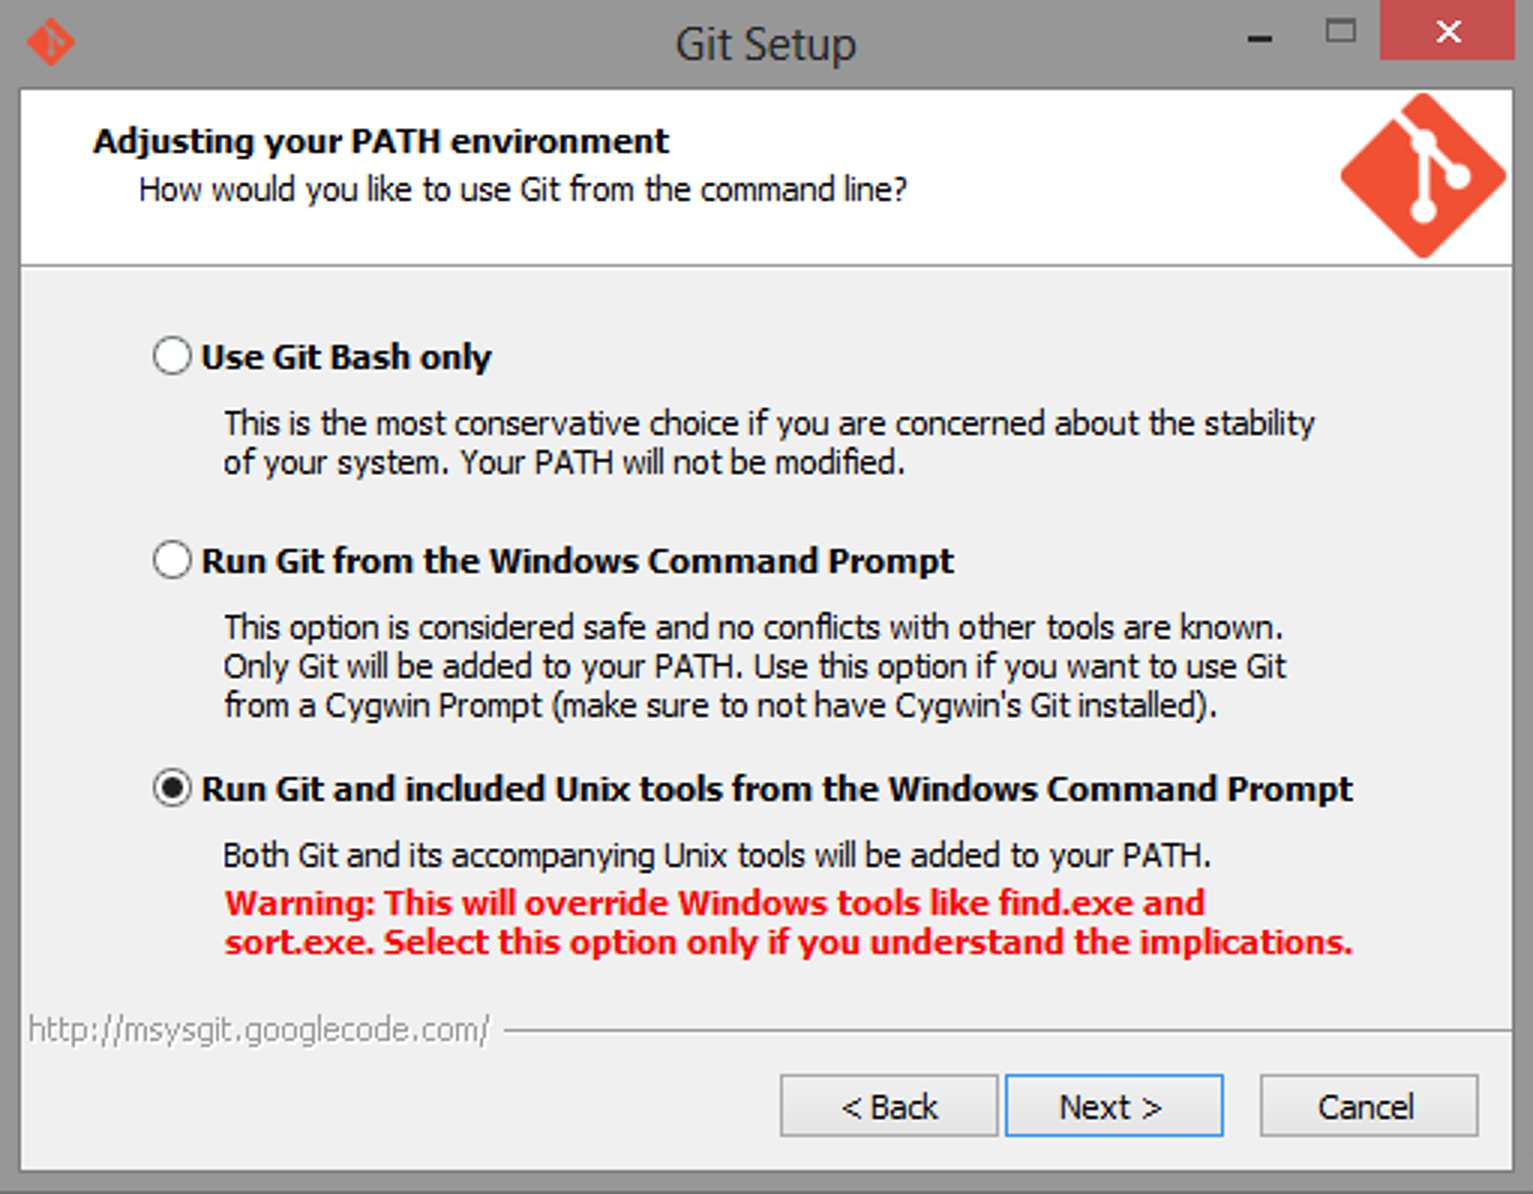
\includegraphics[scale=0.25]{images/git-setup.png} 
 \end{center}
\end{frame}

\begin{frame}
 \begin{center}
    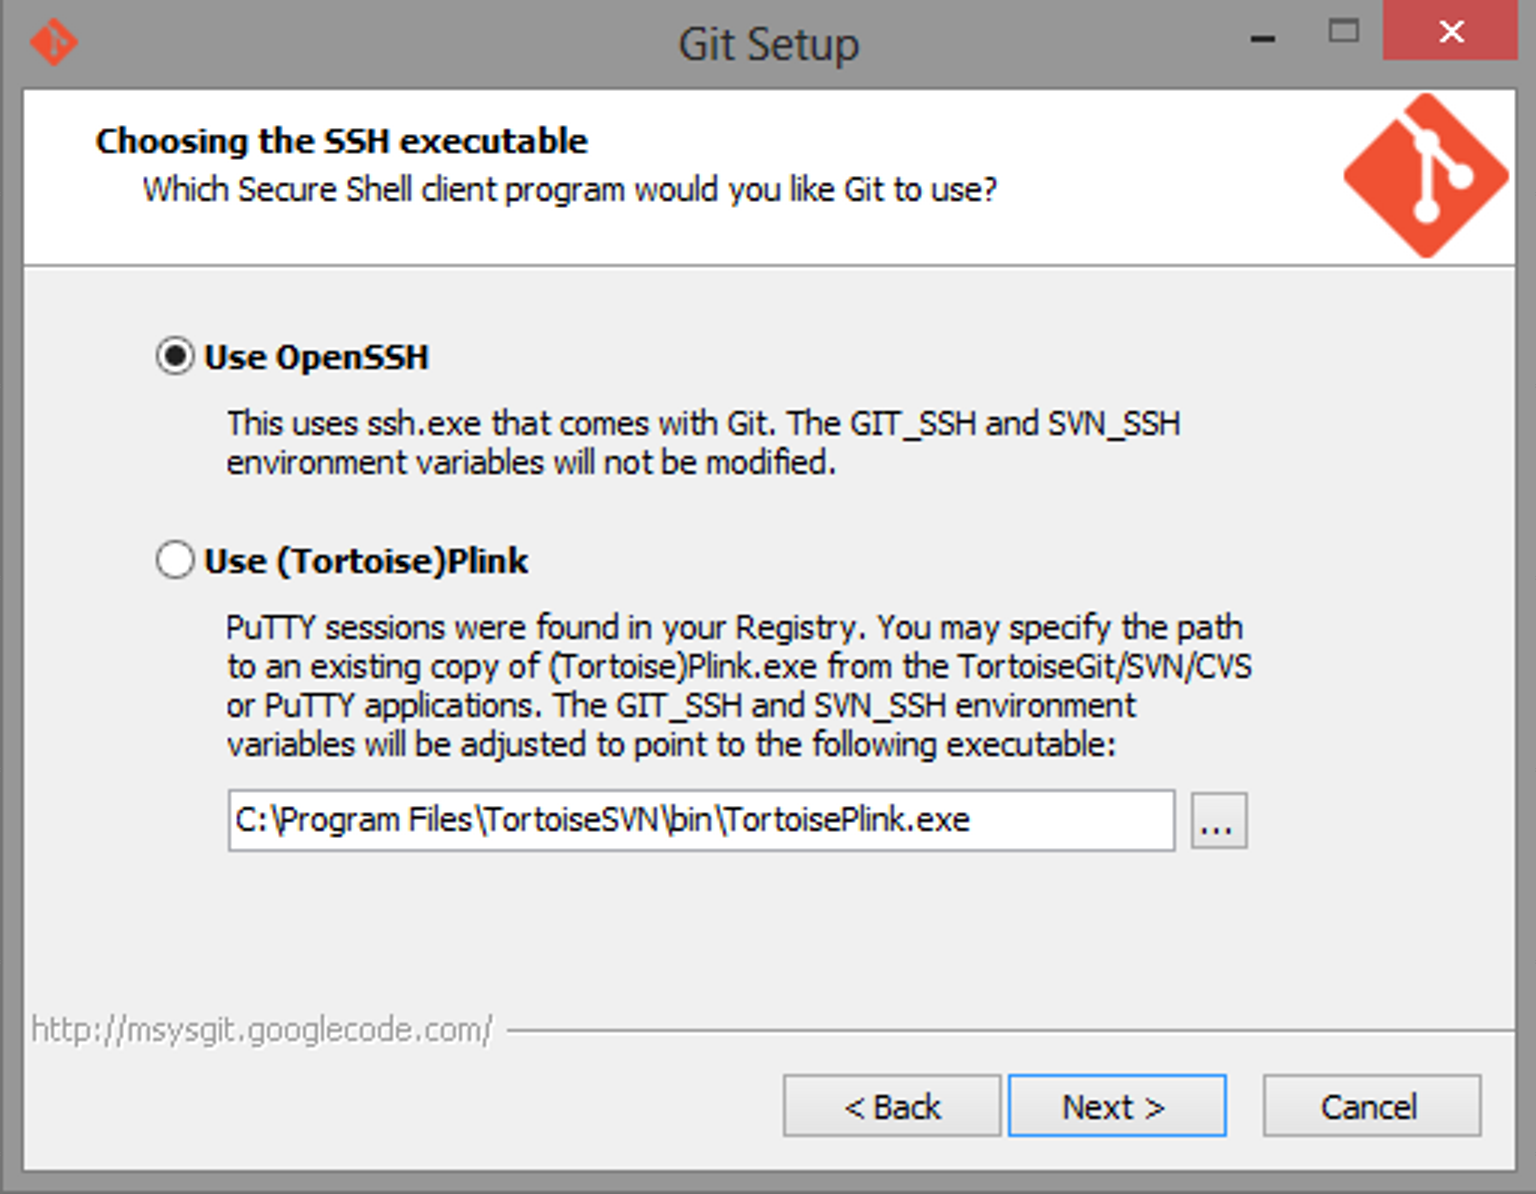
\includegraphics[scale=0.25]{images/git-setup2.png} 
 \end{center}
\end{frame}

\begin{frame}
 \begin{center}
    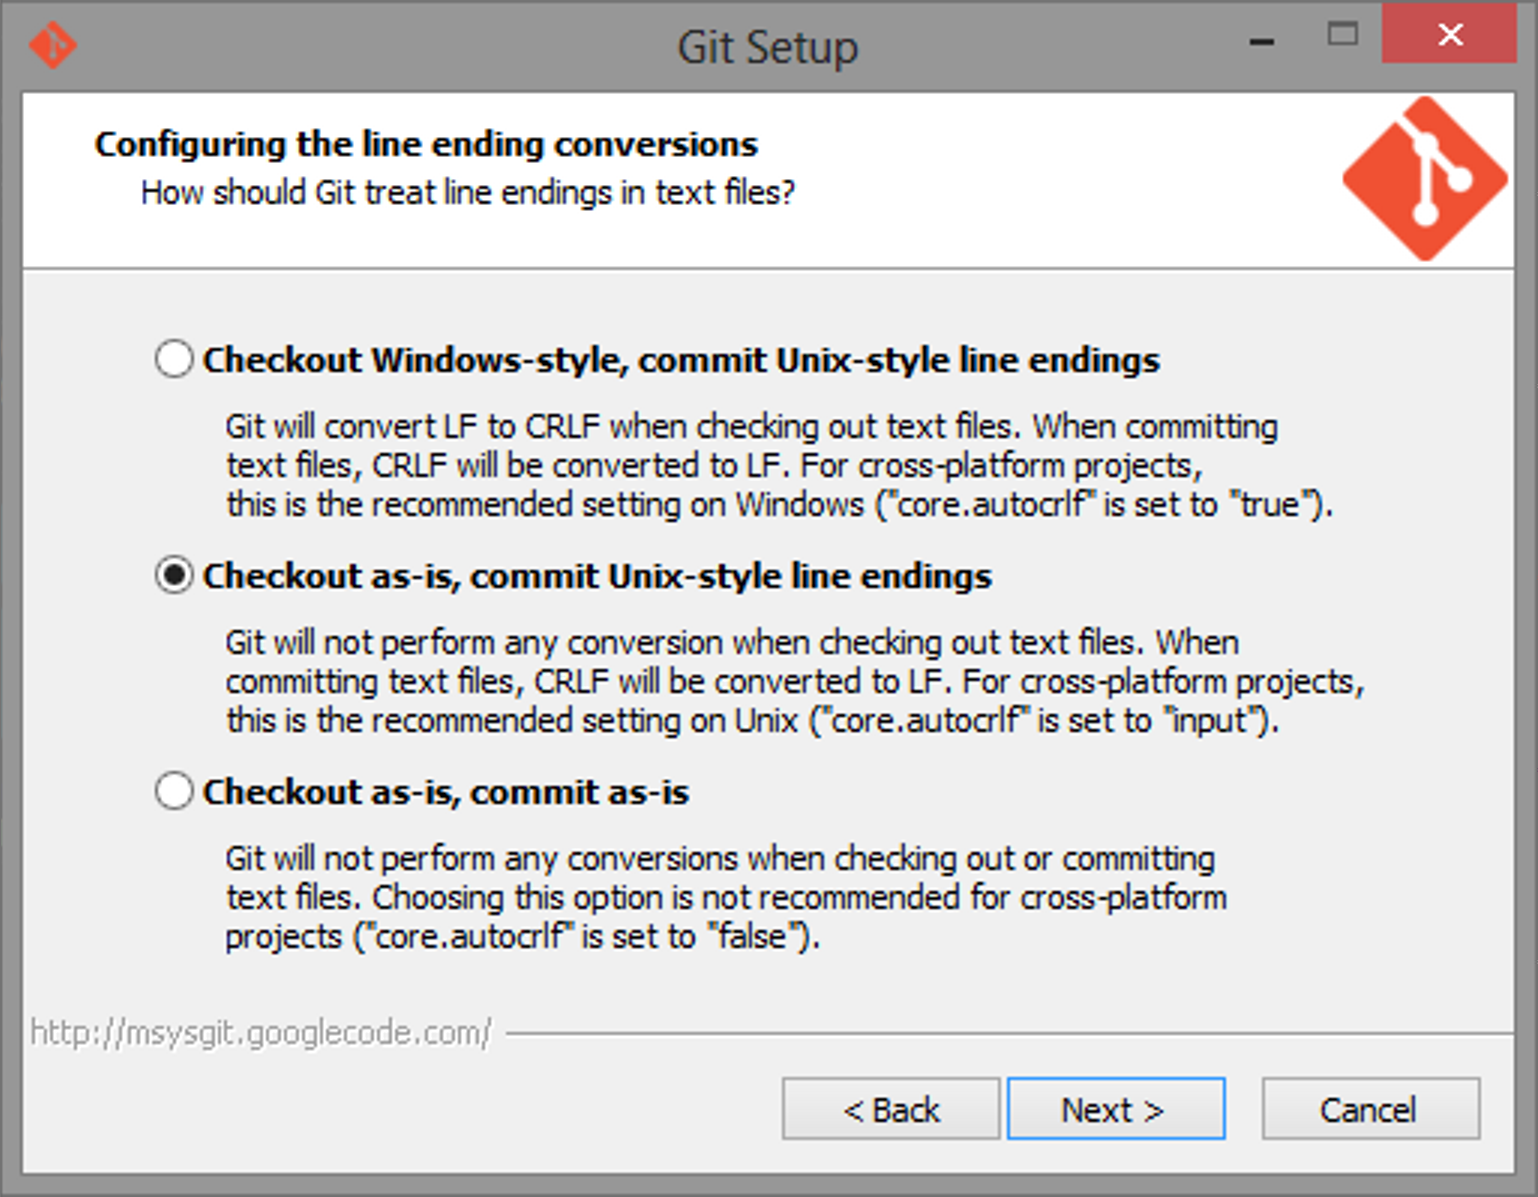
\includegraphics[scale=0.25]{images/git-setup3.png} 
 \end{center}
\end{frame}

%-------------------------------------------------------------------
%                      SSH Einrichtung
%-------------------------------------------------------------------
%
\setbeamercolor{background canvas}{bg=uigreen_dark}
\section{SSH Keygen}
\begin{frame}
  \begin{center}
    \fontHeadII{\cred{SSH}\cgray{Keygen}}
  \end{center}
\end{frame}

\setbeamercolor{background canvas}{bg=uigreen}
\begin{frame}
 \begin{center}
    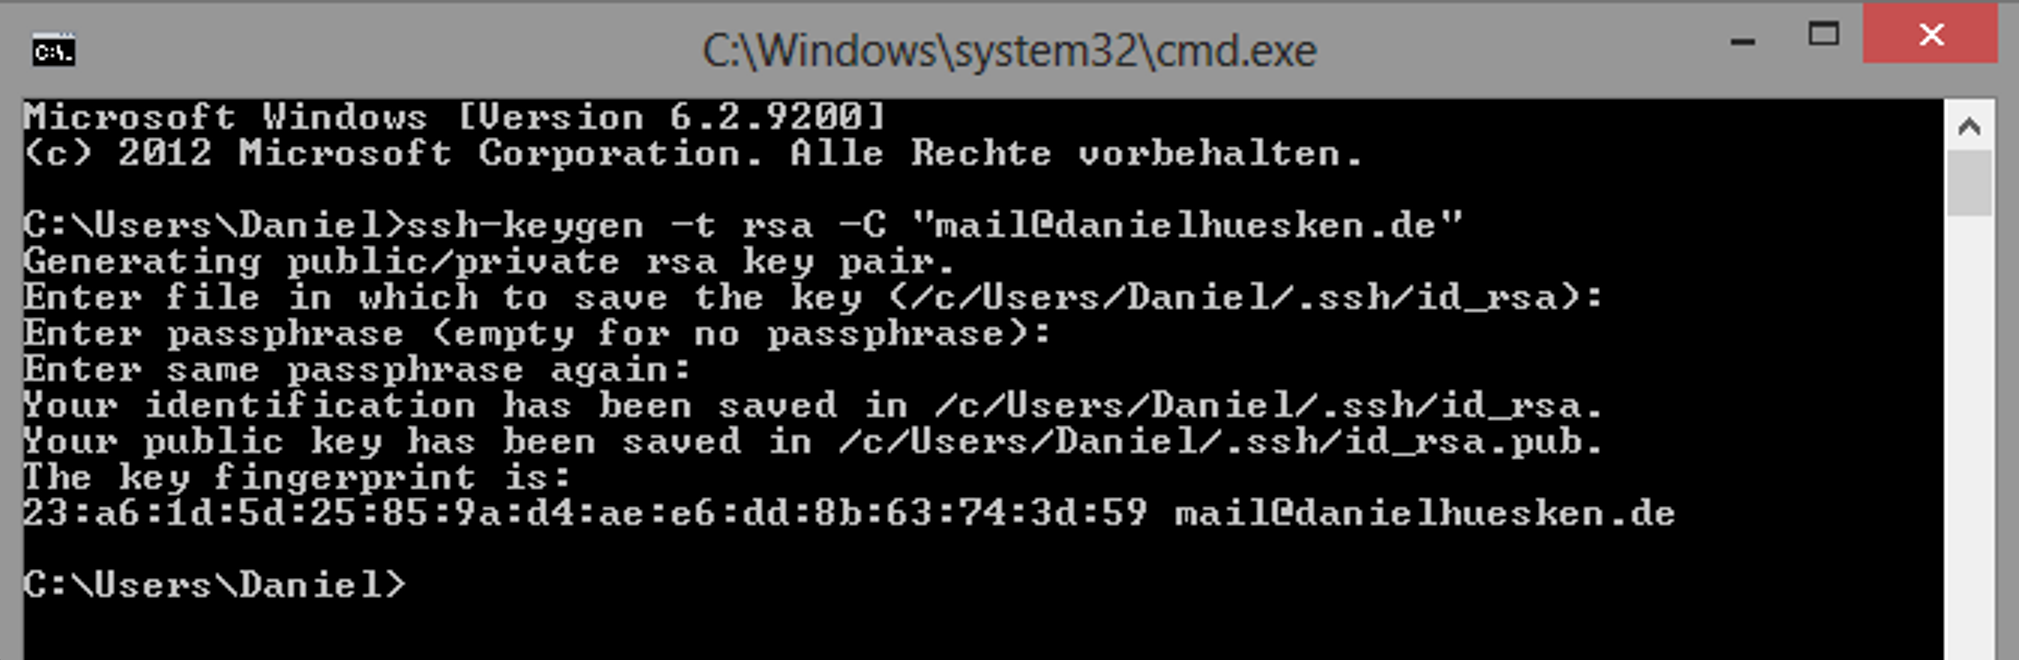
\includegraphics[scale=0.22]{images/ssh.png}
    \fontHeadIV{\cgray{ssh-keygen -t rsa -C \cdark{''mail{@}foo.bar''}}}
 \end{center}
\end{frame}

\begin{frame}
 \begin{center}
    \fontNormal{\cgray{C:\textbackslash{}Users\textbackslash{}<Benutzername>\textbackslash{}.ssh\textbackslash{}}\cdark{id\_rsa.bub}} \\
    \vspace{20pt}
    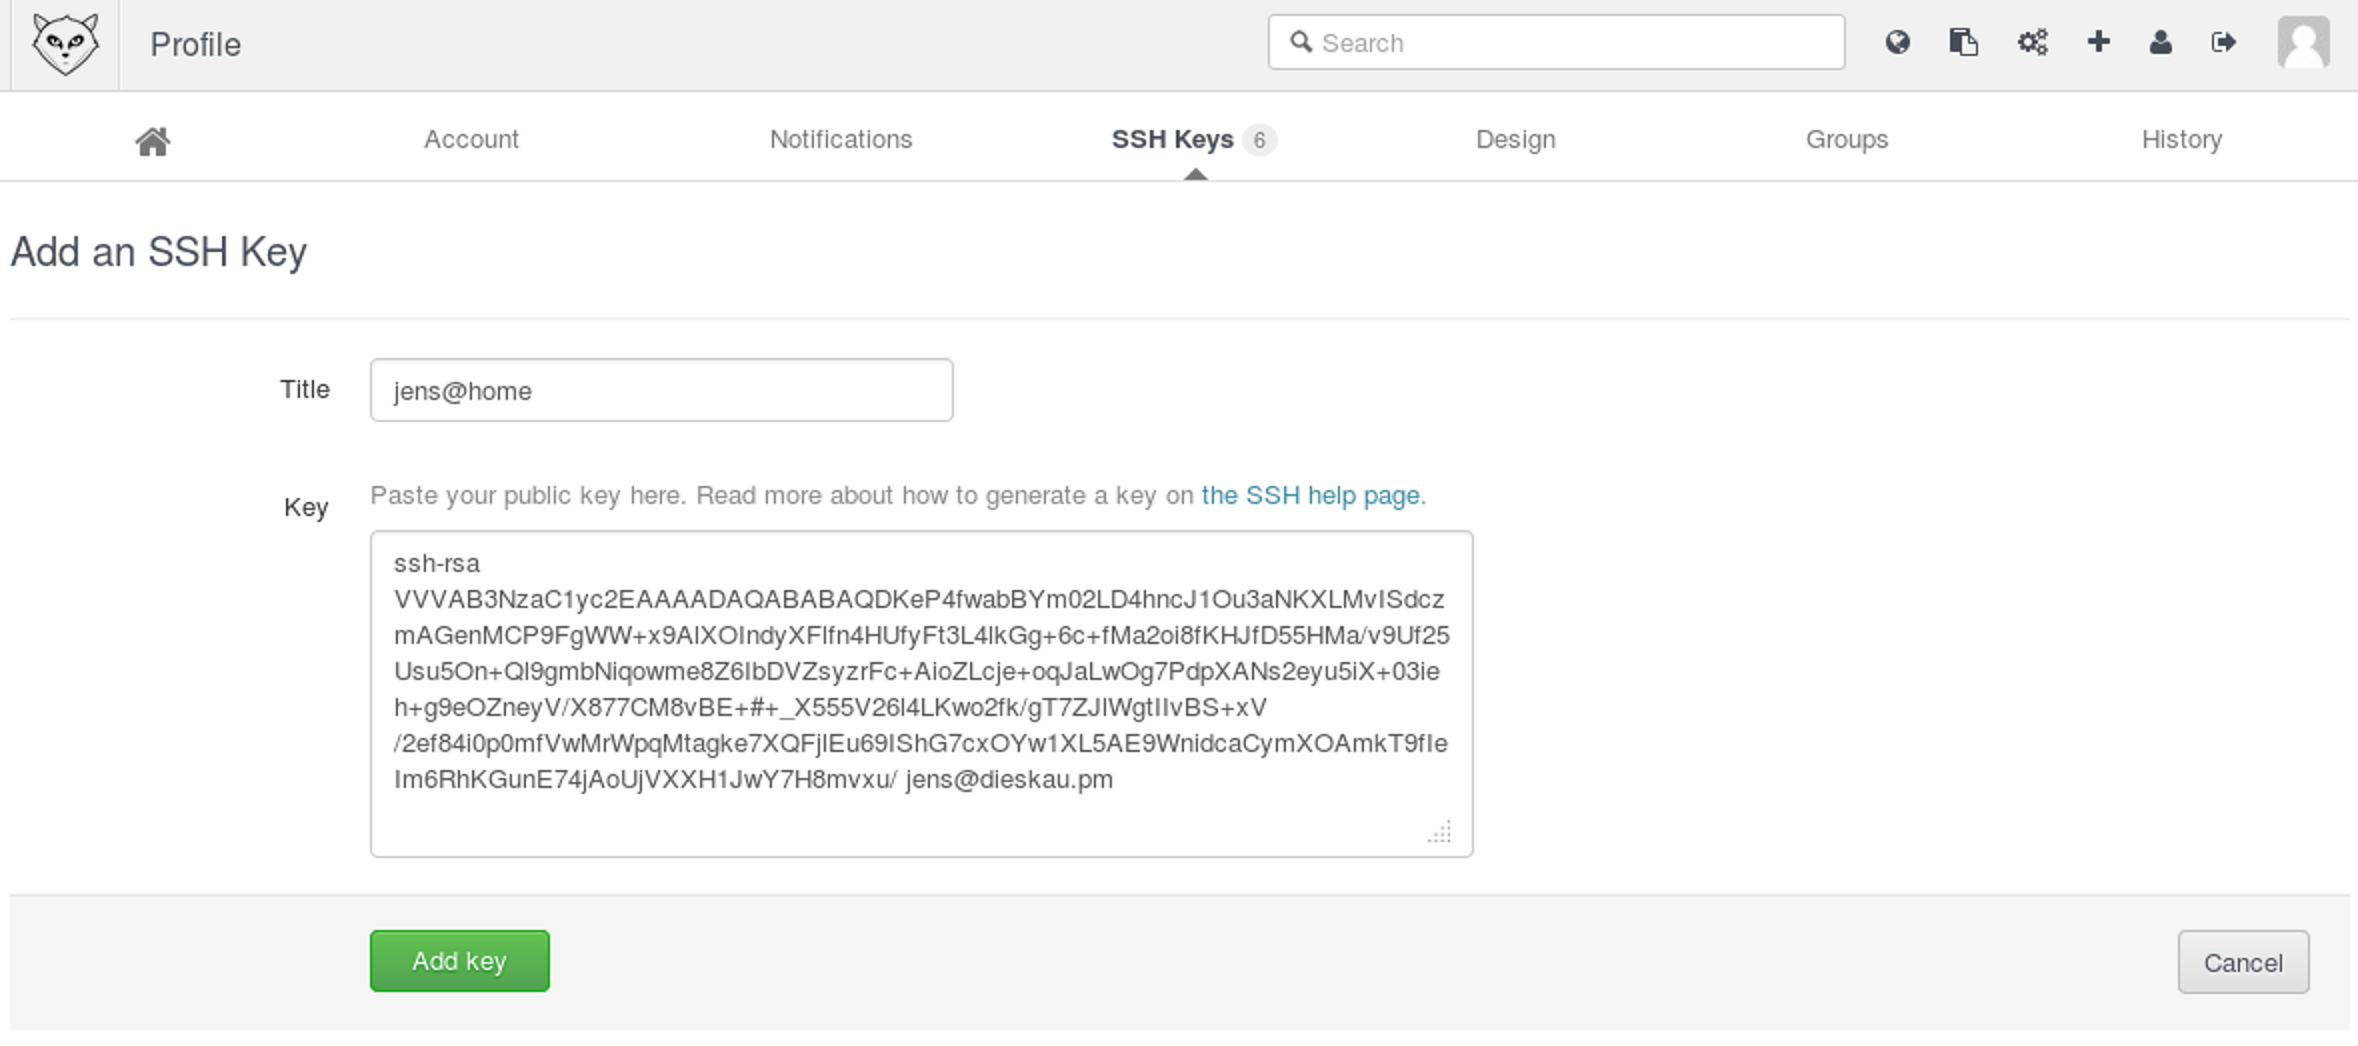
\includegraphics[scale=0.21]{images/github-sshkey.png}

 \end{center}
\end{frame}

\end{document}
